% Start with a high-level overview of your results. Does your work support the claims you listed in section 2.1? Keep this section as factual and precise as possible, reserve your judgement and discussion points for the next "Discussion" section. 

% Go into each individual result you have, say how it relates to one of the claims and explain what your result is. Logically group related results into sections. Clearly state if you have gone beyond the original paper to run additional experiments and how they relate to the original claims. 

% \subsection{Result 1}

% \subsection{Result 2}

% \subsection{Additional results not present in the original paper}

\section{Results} \label{sec:reproduction}

We first test whether the HGN \cite{hgn} can learn the dynamics of the four presented physical systems by measuring the average mean squared error (MSE) of the pixel reconstructions of each predicted frame.
Furthermore, we test the original HGN architecture along with different modifications: a version trained with Euler integration rather than Leapfrog integration (HGN Euler),
%a version trained with no transformer network (HGN no $f_\psi$),
and a version that does not include sampling from the posterior $q_\phi(\bm{z}|\bm{x}_0 ... \bm{x}_T)$ (HGN determ). Since we could not find suitable GECO\cite{geco} hyperparameters, we use a fixed Lagrange multiplier\cite{beta-vae} in all the experiments.
%To test HNN, we use the implementation provided by \cite{hnn} known as pixelHNN.
%Similarly to \cite{hgn}, we test HNN with a modification of the architecture to closely match the HGN (HNN Conv).

\begin{table}[]
    \centering
    \resizebox{\textwidth}{!}{%
    \begin{tabular}{c c c c c c c c c}
     \Xhline{3\arrayrulewidth}
     \textsc{Model} & \multicolumn{2}{c}{\textsc{Mass-spring}} & \multicolumn{2}{c}{\textsc{Pendulum}} & \multicolumn{2}{c}{\textsc{Two-body}} & \multicolumn{2}{c}{\textsc{Three-body}} \\
     & \textsc{Train} & \textsc{Test} & \textsc{Train} & \textsc{Test}& \textsc{Train} & \textsc{Test}& \textsc{Train} & \textsc{Test}\\
    \Xhline{3\arrayrulewidth}
     
    Orig. \textsc{HGN (Euler)} \cite{hgn} & $3.67 \pm 1.09$ & $6.2 \pm 2.69$ & $5.43 \pm 2.53$ & $10.93 \pm 4.32$ & $6.62 \pm 3.93$ & $15.06 \pm 7.01$ & $7.51 \pm 3.49$ & $9.4 \pm 3.92$ \\
    Orig. \textsc{HGN (Determ)} \cite{hgn} & $0.23 \pm 0.23$ & $3.07 \pm 1.06$ & $0.79 \pm 1.24$ & $10.68 \pm 3.19$ & $2.34 \pm 2.3$ & $14.47 \pm 5.24$ & $4.1 \pm 2.05$ & $5.17 \pm 1.96$ \\
    %Orig. \textsc{HGN (No $f_\psi$)} \cite{hgn} & $4.95 \pm 1.71$ & $7.04 \pm 2.55$ & $6.83 \pm 3.29$ & $13.98 \pm 4.94$ & $6.35 \pm 3.86$ & $16.49 \pm 6.6$ & $8.37 \pm 3.13$ & $10.41 \pm 3.72$ \\
    Orig. \textsc{HGN (Leapfrog)} \cite{hgn} & $3.84 \pm 1.07$ & $6.23 \pm 2.03$ & $4.9 \pm 1.86$ & $11.72 \pm 4.14$ & $6.36 \pm 3.29$ & $16.47 \pm 7.15$ & $7.88 \pm 3.55$ & $9.8 \pm 3.72$ \\
     \Xhline{3\arrayrulewidth}
     \textsc{HGN (Euler)} ours & $9.05 \pm 0.02$ & $9.06 \pm 0.05$ & $17.79 \pm 0.06$ & $17.86 \pm 0.13$ & $3.84 \pm 0.01$ & $3.85 \pm 0.02$ & $1.99 \pm 0.01$ & $1.99 \pm 0.01$ \\
     \textsc{HGN (Determ)} ours & $7.10 \pm 0.01$ & $7.10 \pm 0.03$ & $14.11 \pm 0.05$ & $14.14 \pm 0.12$ & $3.92 \pm 0.02$ & $3.93 \pm 0.02$ & $4.14 \pm 0.01$ & $4.13 \pm 0.02$ \\

     \textsc{HGN (Leapfrog)} ours & $7.11 \pm 0.01$ & $7.12 \pm 0.03$ & $14.89 \pm 0.05$ & $14.97 \pm 0.1$ & $3.36 \pm 0.01$ & $3.36 \pm 0.02$ & $8.81 \pm 0.01$ & $8.81 \pm 0.01$ \\
     \Xhline{3\arrayrulewidth}
     \textsc{HGN (Euler)} ours \textit{5-frame inference} & $42.09\pm 0.14$ & $41.98\pm 0.32$ & $47.06\pm 0.17$ & $47.03\pm 0.39$ & $6.46\pm 0.03$ & $6.52 \pm 0.06$ & $8.18 \pm 0.01$ & $8.17 \pm 0.01$ \\
     \textsc{HGN (Determ)} ours \textit{5-frame inference}& $13.00 \pm 0.05$ & $13.04 \pm 0.11$ & $45.06\pm 0.19$ & $44.89 \pm 0.42$ & $10.95\pm 0.02$ & $10.97 \pm 0.05$ & $3.72\pm 0.01$ & $3.72\pm 0.02$ \\
     \textsc{HGN (Leapfrog)} ours \textit{5-frame inference}& $12.15 \pm 0.05$ & $12.21 \pm 0.11$ & $44.29\pm 0.19$ & $44.12\pm 0.42$ & $6.28 \pm 0.03$ & $6.33 \pm 0.06$ & $3.35\pm 0.01$ & $3.35\pm 0.02$ \\
     \Xhline{3\arrayrulewidth}
    
    \end{tabular}}
    \vspace{0.25cm}
    \caption{Average pixel MSE of the reconstruction of a 30-frame rollout sequence on the test and train datasets of the four physical systems presented by \cite{hgn}. All the values are multiplied by $10^4$. We show our results (second and third group) along with the ones reported by the original authors (first group). In the second group, we train to reconstruct the whole inputted sequence (as an autoencoder) and in the third group, we train by inputting only the first 5 frames.}
    \label{tab:reproduction}
\end{table}

Table \ref{tab:reproduction} shows the results of the experiments described previously along with the results of the original authors. As it can be seen, we achieve average pixel reconstruction errors that are similar (30\% avg absolute error w.r.t. the reported values on the test set using Leapfrog integrator) to the ones reported in the original paper when reconstructing the same sequence that is inputted (we call this version \textit{autoencode}).
However, when attempting to train to reconstruct a rollout given only the first 5 frames our model performs poorly, with 107\% average absolute error on the test set, using Leapfrog integrator.
% This might be for several reasons that will be discussed in Sec. \ref{sec:disc}.
%In general, we can observe that our HGN and the proposed modifications learned well on the four physical systems.
% As it can be observed, the results reported by both versions of the HNN are one order of magnitude higher than the four versions of the HGN. Visual inspections of the results provided by HNN show that the network simply learned to output a static image.

\begin{figure}
    \centering
    \begin{subfigure}{.48\textwidth}
        \centering
        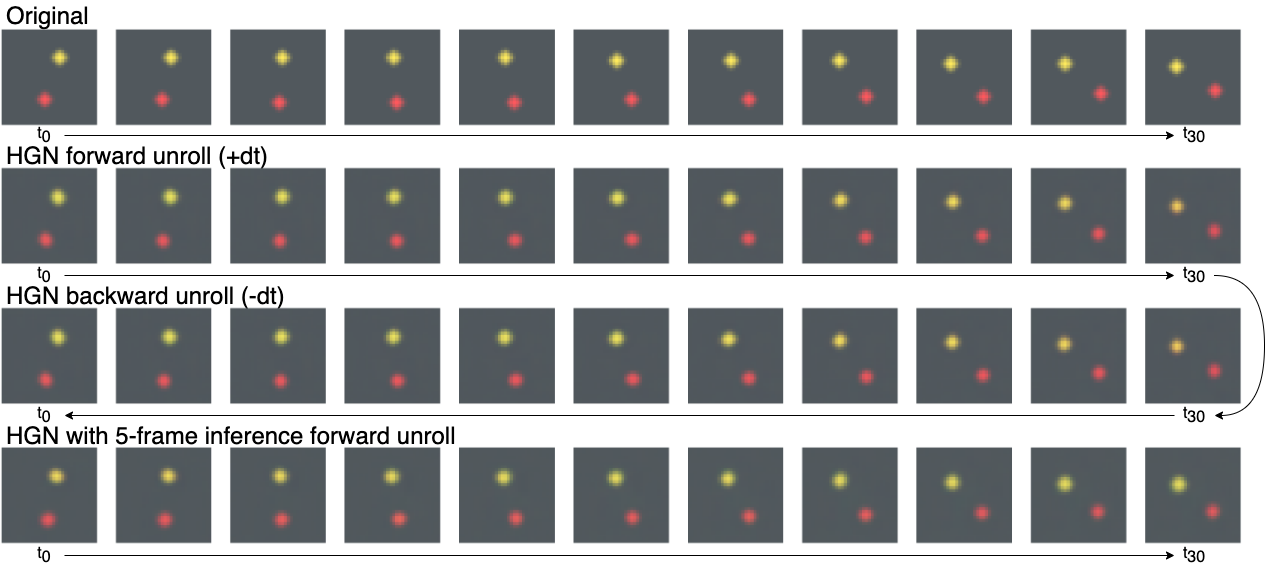
\includegraphics[width=.9\linewidth]{../openreview/pictures/rollout_samples/new_forward_unroll_2_body.png}
        \label{fig:rollout-3-body}
        \caption{}
    \end{subfigure}
    \begin{subfigure}{.48\textwidth}
        \centering
        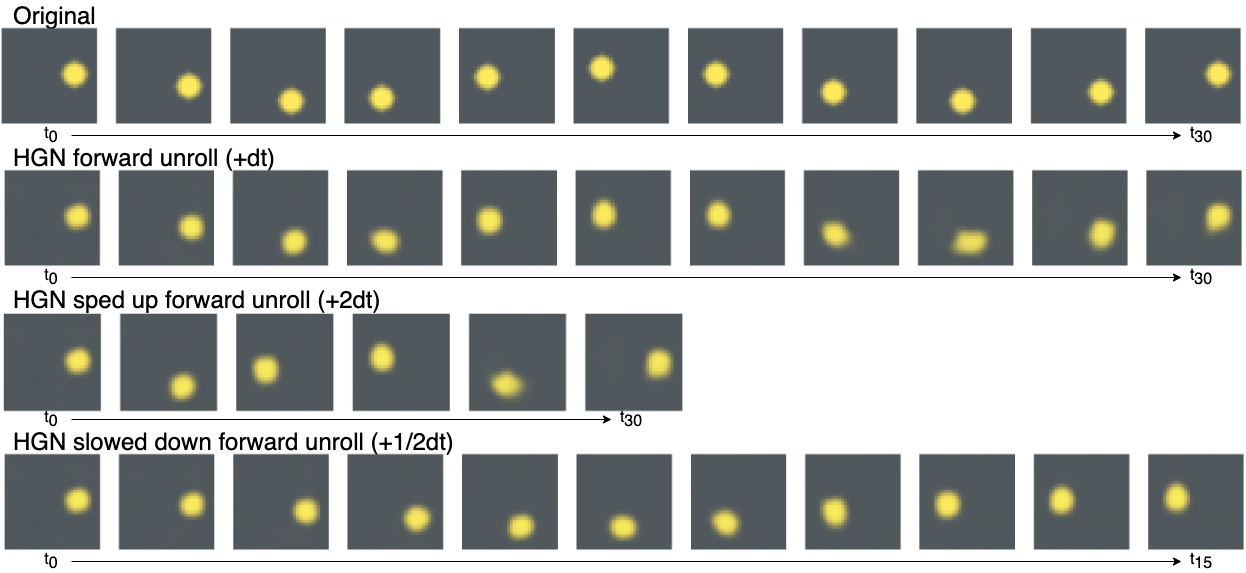
\includegraphics[width=.9\linewidth]{../openreview/pictures/rollout_samples/new_forward_backward_unroll_pendulum.png}
        \caption{}
        \label{fig:rollout-pendulum}
    \end{subfigure}
    \caption{(a) Reconstruction of a sequence of the 2-body system along with a backward unroll of the data from the final state, and a forward rollout of the HGN trained using state inference from the first 5 frames. (b) Reconstruction of a sequence of the pendulum system along with a sped up and a slowed down forward rollout.}
    \label{fig:rollout_back_forth}
\end{figure}

In Figure \ref{fig:rollout_back_forth}, we show some qualitative examples of the reconstructions obtained by the full version of HGN. The model can reconstruct the samples and its rollouts can be reversed in time, sped up, or slowed down by changing the value of the time step used in the integrator. Since the HGN is designed as a generative model, we can sample from the latent space to produce initial conditions and perform their time evolution. We show some rollouts obtained this way in figure \ref{fig:samples}. We observe that our model is only able to generate plausible and diverse samples in the mass-spring dataset.
This behavior is different than the one shown by \cite{hgn} and might be caused by different hyper-parameter configurations in the training procedure or some implementation mistake.
% Later discussion with the authors revealed that they did not input the whole rollout to the encoder but just the first five frames, which was not explained in the paper. Since we received the information too late, we could not run all the experiments again.
% However, we tried this modification in the \textit{mass-spring} dataset, achieving a reconstruction loss of $1.4\times 10^{-3}$, which is very similar to authors results. 


% - The way we assess error: larger bodies with more movement gets more penalized
% - 2-3 bodies move slower and seems better for our model
% - Seems that our hyper-parameter choice is better at physics and theirs better at reconstruction
% - Identify good/bad physiscs and good/bad reconstructions


% Below we comment on the results reported for each environment.

% We takl about mass spring. then talk about pendulum. 
We achieve slightly larger MSE in the autoencode version and significantly larger in the 5-frame inference problem on both the mass-spring and pendulum.
The latter presents roughly double MSE probably because of a wider span of movement.
In general, these two environments show worse results in comparison to two/three-bodies.
For these last cases, our implementation using the \textit{autoencode} setting outperforms the original HGN \cite{hgn}, and when using the \textit{5-frame inference} the results are similar.
As we can see, these two environments show much less average pixel MSE compared to the first ones (almost one order of magnitude).
We believe this may be due to the differences when rendering the instances of each dataset.
The elements appearing in mass-spring and pendulum (represented by a large yellow ball) are larger than the ones present in the two/three bodies (two/three small coloured balls).
Because of this, it would be reasonable to assume that localization errors are more penalized in the first two environments, since the total difference in areas is larger.
Furthermore, the dynamics representing mass-spring and pendulum show faster movements in comparison to two/three-bodies, resulting in being harder to represent with our HGN.
Consequently, we hypothesise the following: larger elements and faster dynamics, produces higher average MSE on our model regardless of the difficulty of the environment physics.
However, this is not the case for the original author's results, who seem to struggle more on the two/three-bodies.
Surprisingly, it seems that our hyperparameter and architecture choices led to poorer reconstruction capabilities (higher MSE) but learning better physics (qualitatively more realistic movements).
% The error gets severely exacerbated when only inputting the first 5 frames of the sequence.

% In fact, 2 bodies are tal tal ,3 bodies are tal tal, and it is because of the previous assumption.






% \begin{itemize}
%     \item \textbf{Mass-spring and Pendulum:}

    
%     In comparison, both environments seem to be harder for us to learn than the multiple bodies ones.
     
%     % Surprisingly, it seems that our hyperparameter and architecture choices let to learning better physics but poorer reconstruction capabilities.

%     \item \textbf{Two-body and Three-body:} As we observe, our implementation using the \textit{autoencode} setting is able to outperform the original HGN \cite{hgn}. On the other hand, when using \textit{5-frame inference}, the results are still comparable. 
    
%     %Although it is hard to draw an exact conclusion on the factors causing these results, we can see the instances represented in the \textit{two/three-body} dataset are smaller compared to the ones in the \textit{mass-spring} or \textit{pendulum} (see Figure \ref{fig:datasets} for reference). Moreover, the dynamics of the \textit{two/three-body} systems are steadier. These two factors
    
%     Autoencode is better than them, 5-frames is similar
%     \item \textbf{Three-body:} Both autoencode and 5-frame better than them. Why?
% \end{itemize}


\begin{figure}
    \centering
    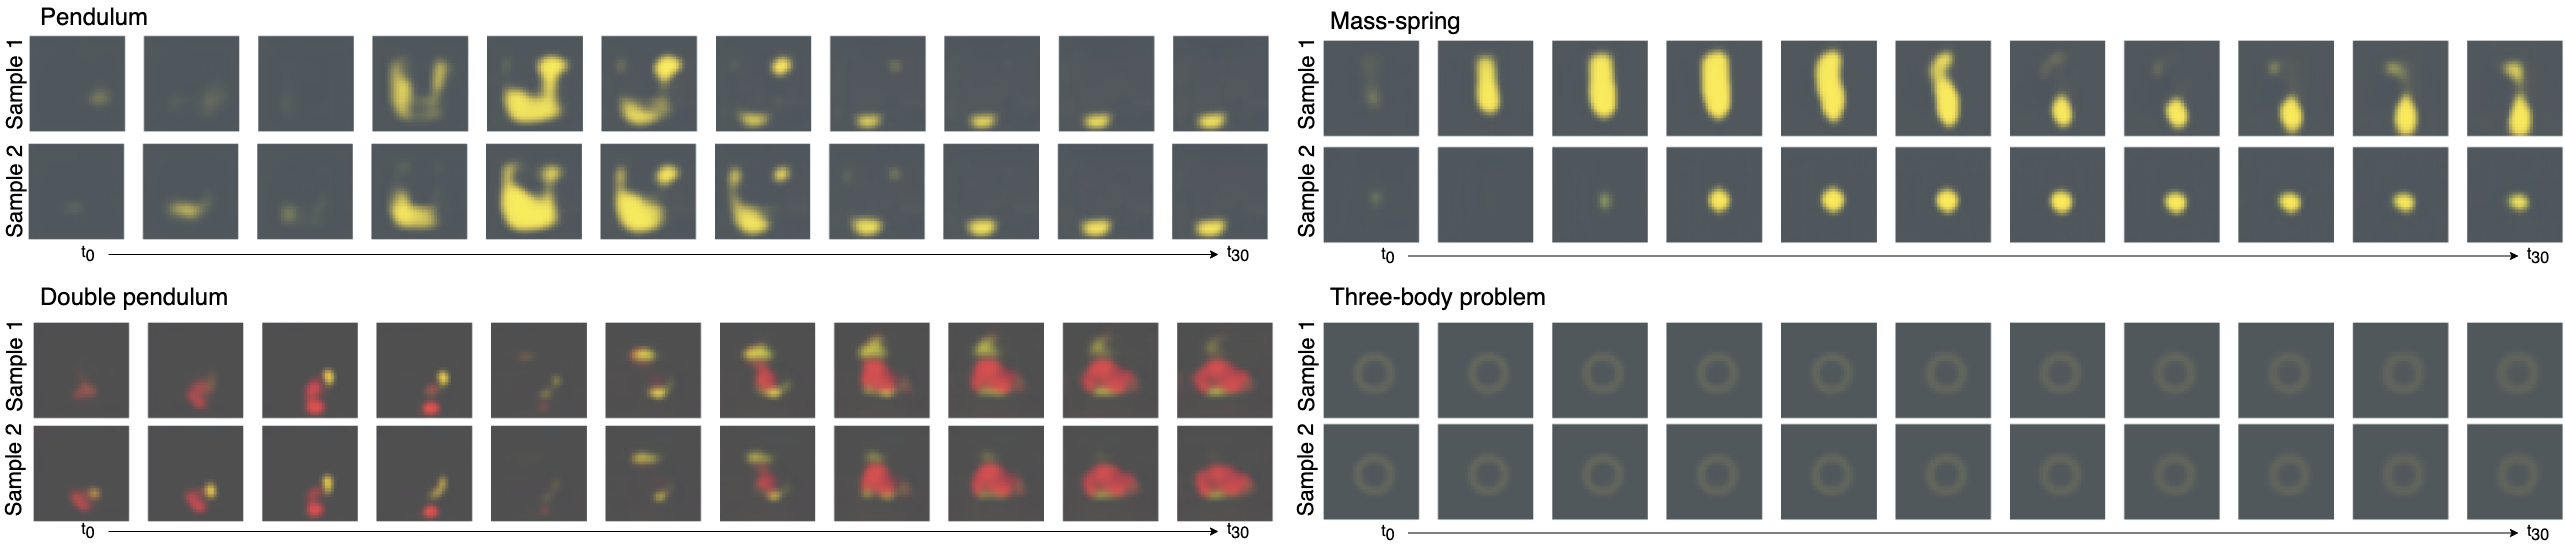
\includegraphics[width=\textwidth]{../openreview/pictures/rollout_samples/new_sampling.png}
    \caption{Examples of sample rollouts from the latent space for different physical systems.}
    \label{fig:samples}
\end{figure}

\subsection{Additional experiments} \label{sec:additional_experiments}

\paragraph{GECO parameter search} \label{sec:hyperparam_search} The paper does not provide the values of GECO \cite{geco} used. In GECO, the Lagrangian multiplier is optimized at each step with a rate $\gamma$.
Figure \ref{fig:geco_search} shows the behavior of GECO for $\gamma \in \{0.1, 0.05, 0.01\}$ in terms of reconstruction loss and KL divergence. Higher values of $\beta$ give a better reconstruction loss but greatly increase the KL divergence. %In our experiments we generally use $\beta = 0.05$, which provides a good trade-off, or $\beta = 0.1$ for environments in which reconstruction is harder (e.g. pendulum).
However, we found that hyperparameters were not consistent among different environments and integrators. For this reason, we do not use GECO in our experiments.
\begin{figure}[]
\minipage{0.5\textwidth}
\centering
  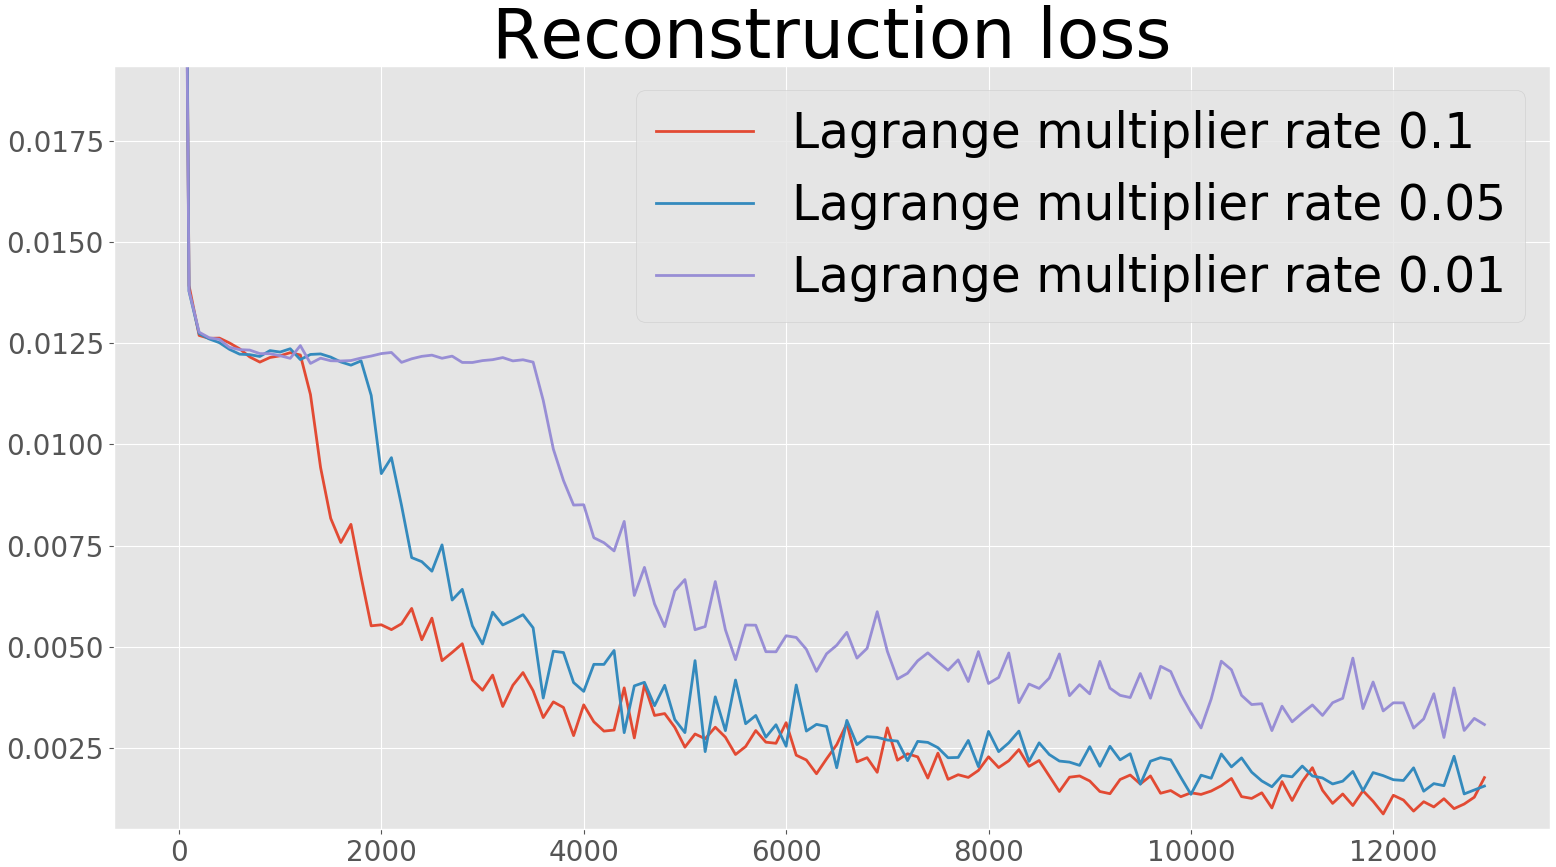
\includegraphics[width=0.8\linewidth]{../openreview/pictures/parameter_comparisons/lagrange_multiplier_comparison_rec_loss.png}
\endminipage\hfill
\minipage{0.5\textwidth}
\centering
  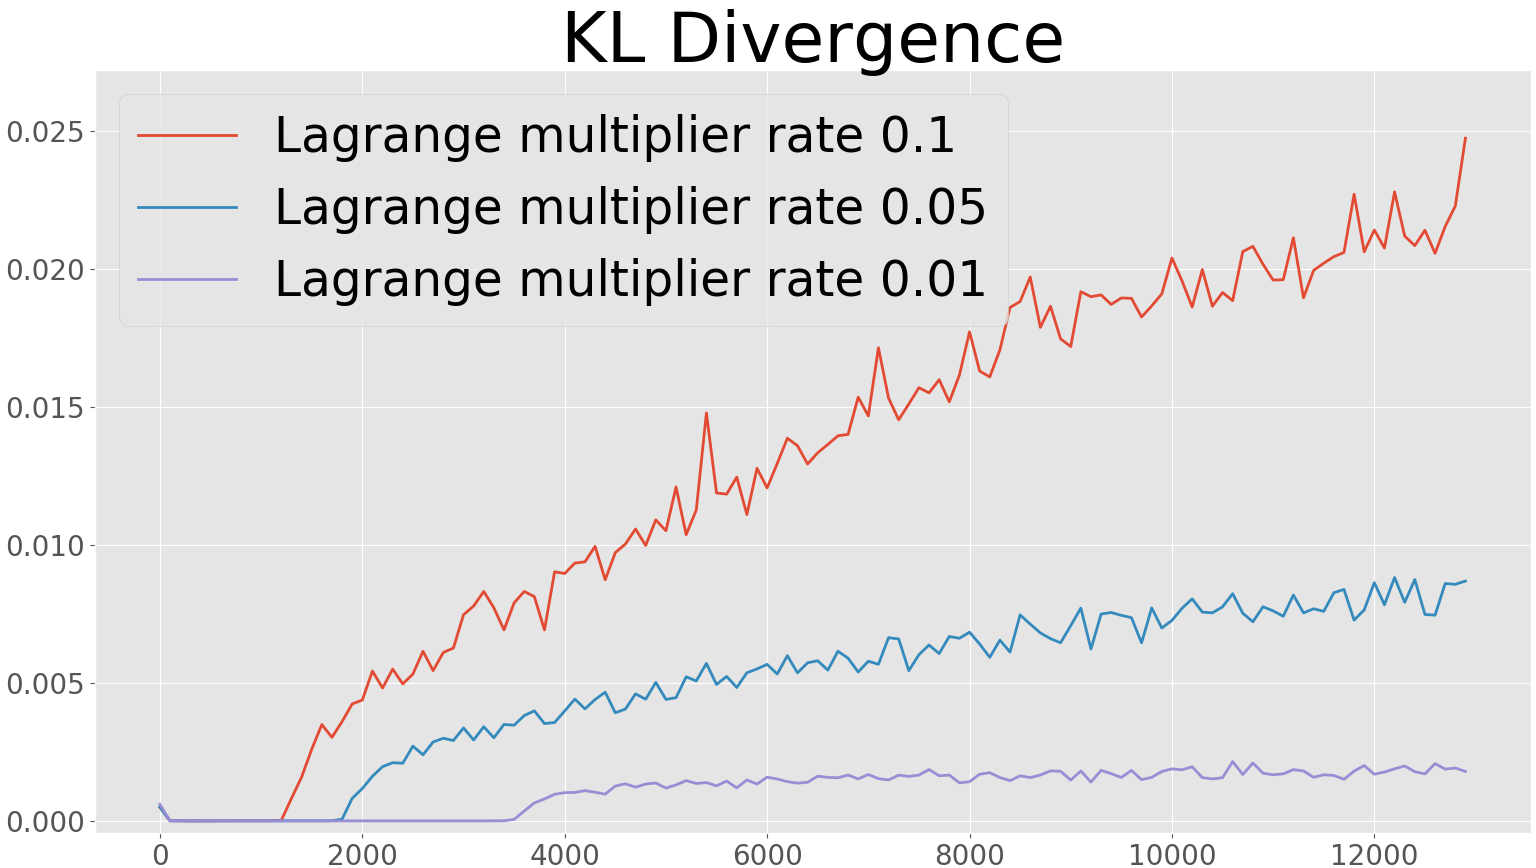
\includegraphics[width=0.8\linewidth]{../openreview/pictures/parameter_comparisons/lagrange_multiplier_comparison_kld.png}
\endminipage
\caption{Reconstruction loss and KL divergence for different GECO parameters in the Pendulum environment.}
\label{fig:geco_search}
\end{figure}


\paragraph{Integrators} \label{sec:integrators}
Performing the integration step is key to generate the time evolution of a rollout given the initial state. 
In the HGN paper \cite{hgn} the system is tested using Euler and Leapfrog integration. We wonder if using higher order integration methods might boost the performance of the rollout generation process.
% The Runge-Kutta integration is only used when training the HNN architecture \cite{hnn}. 
%We observed that one main disadvantage of Euler integration is that its errors accumulate rapidly over longer time periods.
Therefore, we implement and test the HGN architecture with two additional numerical integration methods: the Runge-Kutta's 4th-order integrator \cite{rk4} and the 4th-order Leapfrog integrator (Yoshida's algorithm \cite{yoshida1992symplectic}). Table \ref{tab:integrators} shows a comparison of all four integrators on the Pendulum dataset.
%For this reason other methods that involve more integration steps, such as the fourth-order Runge-Kutta integration (RK4) or the fourth-order Leapfrog (Yoshida's algorithm) \cite{yoshida1992symplectic} have been implemented.
Both Leapfrog and Yoshida are \textit{symplectic} integrators: they guarantee to preserve the special form of the Hamiltonian over time \cite{neal2011mcmc}.
% , at the cost of slower execution.

\begin{table}[]
    \centering

    \begin{tabular}{c c c c c}
     \Xhline{3\arrayrulewidth}
      & \textsc{Euler} & \textsc{Runge-kuta 4} & \textsc{Leapfrog} & \textsc{Yoshida}\\

     \Xhline{3\arrayrulewidth}
     pixel MSE & $17.86 \pm 0.13$ & $76.88 \pm 0.08$ & $14.97\pm 0.10$ & $14.70\pm 0.10$ \\
     $\mathcal{H}$ std & $3.81$ & $0$ & $1961.93$ & $1893.05$\\
     reconstr. time (s) & $0.32$ & $1.89$ & $0.96$ & $1.61$ \\

     \Xhline{3\arrayrulewidth}
    
    \end{tabular}
    \vspace{0.25cm}
    \caption{Comparison between four different integrators used to perform the time evolution in the HGN. The results are measured on the simple pendulum test set. The pixel MSE values have been multiplied by $10^4$.}
    \label{tab:integrators}
\end{table}

Table \ref{tab:integrators} shows the average pixel MSE, the averaged standard deviation of the output of the Hamiltonian network during testing, and the reconstruction time of a single batch ($\texttt{batch}=16$) using the different integration methods that we have described previously. The model has been trained on the simple pendulum dataset. As we can see, the reconstruction time increases when using higher-order integration methods, since they require more integration steps. In general, we see that Euler integration offers a fast and sufficiently reliable reconstruction of the rollouts. Moreover, we observe that the fourth-order symplectic integrator (Yoshida) achieves the best performance. Surprisingly, the symplectic integration methods show more variance in the output of the Hamiltonian networks throughout a single rollout. This behavior is unexpected since using a symplectic integration method should ideally keep the value of the Hamiltonian invariant. We conclude that more experiments need to be performed to guarantee that the implementation of both Leapfrog and Yoshida integration methods are faithful to their formulation.


\paragraph{Integrator modelling} We train the modified architecture of Section \ref{sec:integrator_modelling} on the Pendulum dataset for 5 epochs. The architecture is the same as HGN, but the Hamiltonian Network now outputs $\Delta q$ and $\Delta p$. The average MSE error over the whole Pendulum dataset is $1.485\times 10^{-3}$, while in the test set it is $1.493 \times 10^{-3}$, which are both very close ($\sim \pm 2\%$) to those of autoencoding HGN (see Table \ref{tab:reproduction}). The modified architecture is still capable of performing forward slow-motion rollouts by modifying $\Delta t$. We set $\Delta t' = \frac{\Delta t}{2}$ and we compute the average MSE of the slow-motion reconstruction over 100 rollouts. The modified architecture achieved an error of $8$x$10^{-4}$, while the standard HGN achieved $9$x$10^{-4}$. Note that reconstruction losses are smaller for slow-motion as the images change less between timesteps.



\paragraph{Extra environments}
Apart from the four physical systems presented by \cite{hgn} we test our re-implementation of the HGN with physical systems that do not have a simple Hamiltonian expression. As described previously, these are the damped harmonic oscillator and the double pendulum. On one hand, we are interested in a damped system since it introduces a dissipative term to the equations of motion; a feature that differs from the previous systems. On the other hand, the double pendulum is modelled by a non separable Hamiltonian: $\mathcal{H}(\textbf{q},\textbf{p}) \neq K(\textbf{p}) + V(\textbf{q})$ as described previously. In figure \ref{fig:extra} we show some visual examples of the reconstructions provided by the HGN trained on the two systems. As we can see, HGN is able to reconstruct the damped oscillator with high reliability. Regarding the double pendulum, we observe that the model reconstructs well small oscillations, but fails when the trajectory is too chaotic as expected. The average pixel MSE of the reconstructions of the damped oscillator and the double pendulum are $6.39\cdot 10^{-4}$ and $6.91\cdot 10^{-4}$ respectively. The HGN is able to provide better reconstructions for these systems in comparison to the mass-spring and pendulum systems.

\begin{figure}
    \centering
        \begin{subfigure}{.48\textwidth}
        \centering
        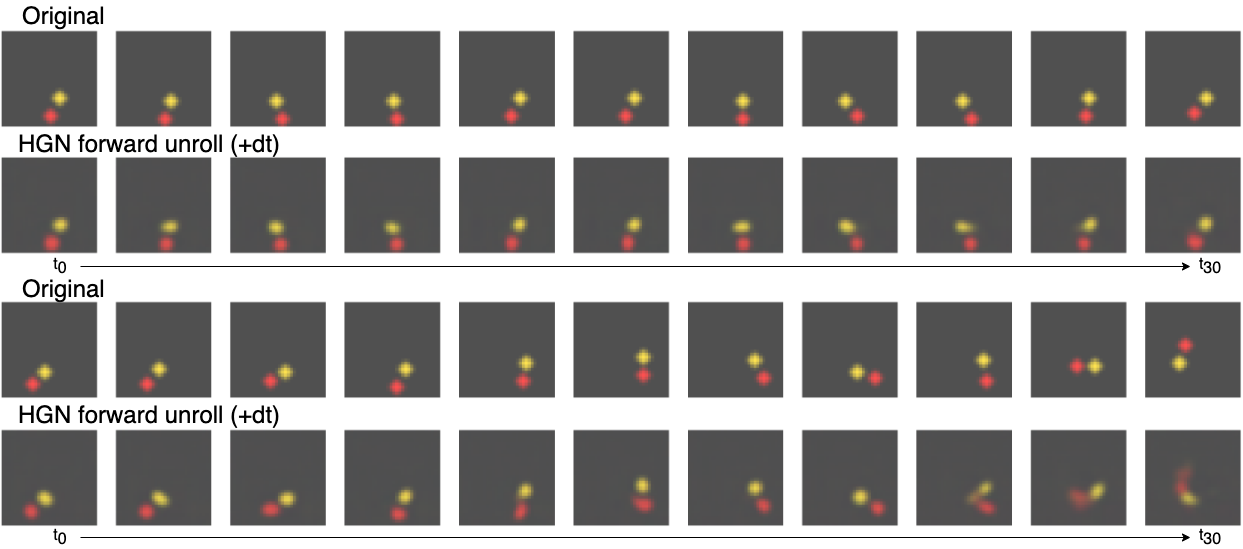
\includegraphics[width=\linewidth]{../openreview/pictures/rollout_samples/new_chaotic_pendulum_rollouts.png}
        \label{fig:a}
    \end{subfigure}
    \begin{subfigure}{.48\textwidth}
        \centering
        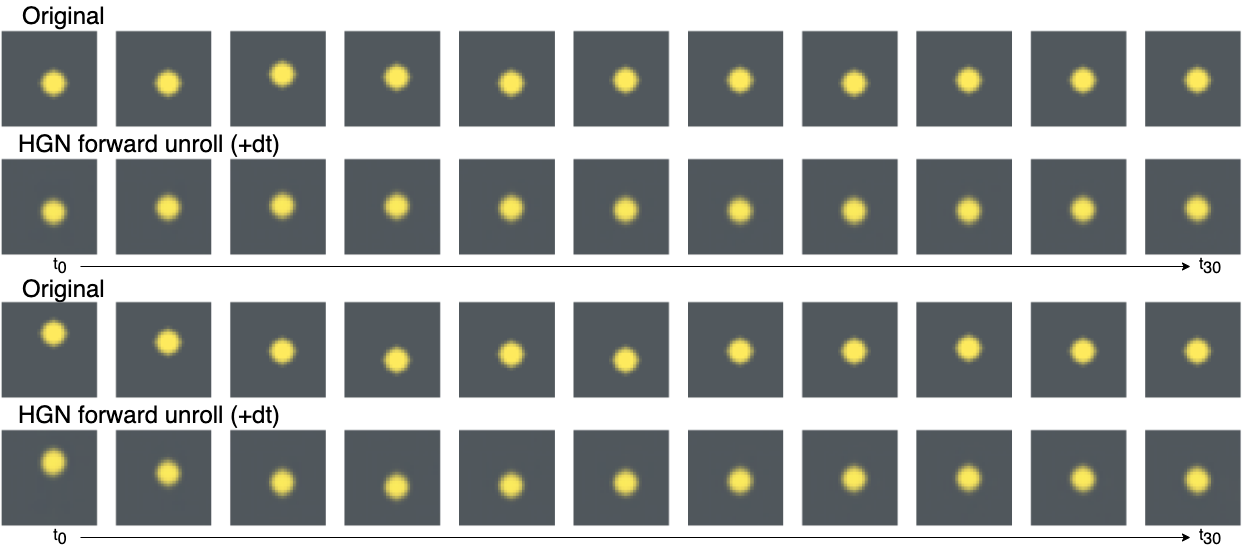
\includegraphics[width=\linewidth]{../openreview/pictures/rollout_samples/new_damped_spring_sample_rollout.png}
        \label{fig:b}
    \end{subfigure}
    \caption{Examples of reconstructions of the double pendulum (left) and the damped harmonic oscillator (right).}
    \label{fig:extra}
\end{figure}
